% =============================================================================
% NL2Semantic2SQL: A Cross-Domain Framework for Natural Language to SQL over
% Geospatial and Enterprise Data Warehouses
% Initial-review LaTeX draft (single column, generic article class).
% Updated after first-round internal review comments.
% =============================================================================
\documentclass[11pt]{article}

\usepackage[margin=1in]{geometry}
\usepackage{times}
\usepackage{amsmath,amssymb}
\usepackage{graphicx}
\usepackage{booktabs}
\usepackage{multirow}
\usepackage{caption}
\usepackage{subcaption}
\usepackage{enumitem}
\usepackage{url}
\usepackage[hidelinks]{hyperref}
\usepackage{tikz}
\usetikzlibrary{positioning,arrows.meta,shapes.geometric,fit,calc}

\title{NL2Semantic2SQL: A Cross-Domain Framework for Natural Language to SQL over Geospatial and Enterprise Data Warehouses}
\author{Anonymous Author(s) \\ \textit{Affiliation withheld for review}}
\date{}

\begin{document}
\maketitle

% =============================================================================
\begin{abstract}
% =============================================================================
Natural language to SQL (text-to-SQL) has advanced rapidly with large language models, yet most existing systems and benchmarks focus on conventional relational databases and provide limited coverage of executable geospatial SQL. Geospatial databases introduce additional challenges, including geometry-aware schema grounding, spatial predicates, coordinate reference systems, and domain-specific operators such as intersection, buffer, area, and distance calculations. At the same time, practical data platforms increasingly require a single interface that can support both geospatial and non-geospatial warehouse queries. In this work, we present NL2Semantic2SQL, a cross-domain framework that combines semantic-layer grounding, intent-conditioned routing, schema-aware prompt construction, few-shot retrieval, SQL postprocessing, and execution-time self-correction to support natural-language querying over both GIS and conventional warehouse data. To evaluate the geospatial side of this problem, we construct a pilot GIS-oriented benchmark with execution-based evaluation and a separate robustness suite, and we further assess cross-domain generalization on a 500-question warehouse benchmark derived from BIRD mini\_dev. After adding Phase~A intent-conditioned grounding, the full pipeline outperforms the baseline on both spatial EX (0.933 vs.\ 0.867) and robustness (0.800 vs.\ 0.000), yielding a combined pilot score of 0.900 vs.\ 0.650. On the 500-question BIRD benchmark, the full pipeline reaches parity with the baseline (0.450 vs.\ 0.458), confirmed by McNemar $p=0.8151$. An intent-class ablation shows that the main contribution of intent routing is preventing spurious LIMIT injection on non-preview queries and enabling KNN-specific operator rules. A preliminary cross-lingual experiment on Chinese translations of BIRD questions further shows that multilingual alias registration supports cross-lingual querying with a four-percentage-point loss relative to the English warehouse run. These findings demonstrate both the promise and the limitations of unified semantic-to-SQL architectures across heterogeneous database domains, and they suggest that future cross-domain text-to-SQL systems must explicitly account for language, schema, and operator heterogeneity rather than assuming a single grounding strategy will generalize uniformly.
\end{abstract}

\noindent\textbf{Keywords:} text-to-SQL; natural language interface; geospatial database; PostGIS; semantic layer; large language model; cross-domain generalization; cross-lingual evaluation.

% =============================================================================
\section{Introduction}
\label{sec:intro}
% =============================================================================

Natural language to SQL has become one of the most active application directions of large language models, because it offers a direct interface between end users and structured data repositories. Recent advances have substantially improved performance on public benchmarks such as Spider~\cite{yu2018spider} and BIRD~\cite{li2023bird}, demonstrating that modern language models can often synthesize executable SQL from natural-language questions under conventional relational settings. However, most existing text-to-SQL systems and evaluation datasets are designed for general-purpose relational databases, where the principal challenges lie in schema linking, join reasoning, aggregation, and nested query construction. By contrast, real-world geospatial database applications introduce additional semantic and operational complexity that is largely absent from these benchmarks. In geospatial settings, queries frequently involve geometry-aware schema grounding, spatial predicates, coordinate reference systems, topological relations, and spatial measurement operators such as area, distance, intersection, and buffering. These characteristics make geospatial text-to-SQL a substantially different problem rather than a simple extension of general warehouse querying.

This mismatch creates a practical and scientific gap. From a practical perspective, many operational data platforms must serve both geospatial and non-geospatial workloads through a unified natural-language interface. A user may ask one question about land-use overlap, another about building proximity, and a third about tabular business statistics in the same system. From a scientific perspective, however, existing studies rarely examine whether a single semantic grounding architecture can support these heterogeneous query types without severe domain bias. Most prior work either optimizes for conventional warehouse-style SQL generation or focuses on domain-specific geospatial systems without evaluating transferability beyond the GIS context. As a result, it remains unclear which components of a semantic-to-SQL pipeline generalize across domains and which components encode assumptions that are beneficial in one setting but harmful in another.

The challenge is especially pronounced at the grounding stage. In conventional text-to-SQL systems, schema linking is often framed as the task of aligning user expressions with table names, column names, or retrieved schema snippets. In geospatial systems, this step is more complicated because the model must additionally recognize geometry-bearing attributes, infer relevant spatial operators, respect spatial reference transformations, and distinguish between topological, metric, and aggregation-based reasoning. At the same time, aggressive domain-specific grounding strategies can introduce unintended bias when transferred to non-geospatial databases. A system tuned for Chinese GIS terminology, spatial operator hints, and geometry-aware rules may perform strongly on spatial benchmarks while underperforming on English warehouse benchmarks if its semantic retrieval mechanisms fail to adapt to differences in language, schema naming, and operator distributions. Understanding this tension is critical for building robust cross-domain natural-language interfaces to structured data.

To address this problem, we present \textbf{NL2Semantic2SQL}, a cross-domain framework that integrates semantic-layer grounding, schema-aware context construction, few-shot retrieval, SQL postprocessing, and execution-time self-correction into a unified natural-language-to-SQL pipeline. Rather than treating SQL generation as a single-step prompting problem, the framework first resolves semantic context, then assembles structured schema evidence, and finally performs constrained SQL generation with post-hoc correction. The design is motivated by the observation that GIS queries and non-GIS warehouse queries share a common need for semantic disambiguation, but differ substantially in the kinds of evidence and constraints that must be surfaced to the model. Our framework therefore aims to preserve a unified architecture while allowing domain-specific grounding signals to be incorporated explicitly rather than implicitly.

To evaluate the geospatial side of the problem, we further construct a pilot GIS-oriented benchmark with execution-based evaluation, spatial-operator coverage, and varying query complexity. The benchmark is designed to capture the characteristics missing from mainstream text-to-SQL datasets, including spatial selection, overlap analysis, buffering, spatial aggregation, and geometry-sensitive reasoning. We then complement this benchmark with cross-domain evaluation on a warehouse-oriented dataset derived from BIRD mini\_dev~\cite{li2023bird}, enabling a direct comparison between GIS and non-GIS scenarios under the same evaluation harness. This dual-track setting allows us to move beyond a simple ``does it work?'' question and instead ask a more informative scientific question: how does a unified semantic-to-SQL architecture behave when confronted with two structurally different database domains?

\medskip
\noindent\textbf{Contributions.} Our contributions are threefold:
\begin{enumerate}[leftmargin=*]
  \item We propose a unified \textbf{NL2Semantic2SQL framework} for cross-domain querying over geospatial and conventional warehouse databases. The framework provides a single semantic-grounding pipeline that adapts its grounding evidence to the target domain (GIS vs.\ warehouse) without retraining or model swapping.
  \item We construct a \textbf{pilot GIS-oriented text-to-SQL benchmark} and explicitly separate ordinary spatial-SQL execution from robustness/safety evaluation, avoiding the common pitfall of conflating refusal behavior with execution accuracy. Combined with a 50-question subset of BIRD mini\_dev, this yields a dual-track protocol that is executable, auditable, and useful for cross-domain error analysis.
  \item Through cross-domain experiments, three pipeline configurations (baseline, prompt-refined full pipeline, and MetricFlow-augmented full pipeline), and a preliminary cross-lingual stress test, we show that semantic grounding provides clear gains for robustness and geometry-sensitive failures in GIS, while warehouse-side parity requires explicit fact/dimension/entity metadata. These results sharpen the decomposition of the cross-domain text-to-SQL problem rather than claiming a uniformly superior end-to-end system.
\end{enumerate}

The remainder of this paper is organized as follows. Section~\ref{sec:related} reviews related work on text-to-SQL with LLMs, public benchmarks, geospatial NL interfaces, semantic layers, and cross-domain/cross-lingual generalization. Section~\ref{sec:method} formalizes the cross-domain text-to-SQL problem and details the proposed three-stage architecture. Section~\ref{sec:experiments} presents the dual-track evaluation, including dataset construction, experimental setup, per-track results, case studies, and reproducibility notes. Section~\ref{sec:discussion} discusses interpretation limits and future work. Section~\ref{sec:conclusion} concludes.

% =============================================================================
\section{Related Work}
\label{sec:related}
% =============================================================================

\subsection{Text-to-SQL with large language models}

The application of large language models to text-to-SQL has progressed rapidly through increasingly sophisticated prompt-engineering strategies. Early in-context learning approaches demonstrated that LLMs could generate executable SQL from natural-language questions when provided with schema descriptions and example query pairs~\cite{yu2018spider,rajkumar2022evaluating}. DIN-SQL~\cite{pourreza2023dinsql} introduced a decomposed prompting pipeline that separates schema linking, query classification, and SQL generation into distinct stages, with self-correction as a post-generation step. DAIL-SQL~\cite{gao2024dail} systematized few-shot example selection based on SQL skeleton similarity and achieved strong results on the Spider benchmark with minimal token cost. C3~\cite{dong2023c3} explored zero-shot ChatGPT-based text-to-SQL with calibrated bias correction, illustrating a complementary line of prompt-engineered solutions that does not rely on hand-crafted few-shot examples. Our framework shares the decomposition philosophy of DIN-SQL but adds an explicit semantic layer as a structured intermediary between the user question and the schema, rather than relying solely on prompt-level schema linking.

\subsection{Benchmarks for text-to-SQL}

Spider~\cite{yu2018spider} established the standard cross-database text-to-SQL benchmark with execution-based evaluation, introducing the challenge of generalizing across unseen database schemas. BIRD~\cite{li2023bird} extended this setting to larger, more realistic databases with value-aware evaluation and difficulty stratification, revealing that LLM performance degrades substantially on complex aggregation and multi-hop join queries. Spider~2.0~\cite{lei2025spider2} further expanded the scope to include enterprise-style workflows such as dbt transformations and dialect variations. BEAVER~\cite{chen2024beaver} specifically targets enterprise data warehouses with private schemas and complex business logic, showing that state-of-the-art models achieve near-zero accuracy on truly private enterprise data. Our work is motivated by a complementary gap: mainstream text-to-SQL benchmarks provide limited coverage of executable geospatial SQL, and none assess cross-domain transfer between GIS and warehouse query semantics in a single evaluation protocol.

\subsection{Geospatial natural language interfaces}

Natural language interfaces to geospatial databases have a distinct research lineage from general text-to-SQL. Early systems focused on template-based spatial query construction for specific GIS applications~\cite{punjani2018geospatial}. More recent work has explored using LLMs for spatial reasoning and geographic knowledge extraction~\cite{mai2023foundation}, but systematic evaluation of text-to-SQL capabilities over PostGIS or spatially-extended relational databases remains scarce. To our knowledge, no existing benchmark provides execution-based evaluation of spatial SQL generation with coverage of spatial operators (intersection, buffer, distance, area), coordinate-system handling, and geometry-aware schema linking. Our GIS benchmark is designed to fill this gap.

\subsection{Semantic layers and schema grounding}

The concept of a semantic layer as an intermediary between analytical queries and raw database schemas originates from business-intelligence tools and has been formalized in frameworks such as MetricFlow~\cite{metricflow} and dbt's semantic layer. These systems define entities, dimensions, measures, and metrics as declarative metadata that governs how joins and aggregations should be constructed. In the text-to-SQL context, semantic layers offer a principled way to provide LLMs with structured evidence about schema semantics rather than requiring the model to infer join paths and aggregation rules from raw DDL alone. Our framework adapts this concept for cross-domain use, combining GIS-specific annotations (geometry types, SRIDs, spatial operators) with warehouse-style entity-relationship metadata to support both query domains through a unified grounding architecture.

\subsection{Cross-domain and cross-lingual text-to-SQL}

Cross-domain generalization has been studied primarily through zero-shot transfer across database schemas within the same linguistic and operator domain~\cite{yu2018spider,li2023bird}. Cross-lingual text-to-SQL, where questions are posed in one language over schemas defined in another, has received less systematic attention, though multilingual benchmarks such as CSpider~\cite{min2019cspider} demonstrate that language mismatch introduces additional schema-linking challenges. Our work extends the cross-domain dimension beyond schema variation to include operator heterogeneity (spatial vs.\ tabular) and language heterogeneity (Chinese questions over English warehouse schemas), providing a more comprehensive view of the generalization landscape.

% =============================================================================
\section{Method}
\label{sec:method}
% =============================================================================

\subsection{Problem formulation}

We formulate cross-domain natural language to SQL as the task of translating a user question $q$ into an executable SQL statement $s$ over heterogeneous structured databases that may belong to either geospatial or conventional warehouse domains. Let $S$ denote the executable schema representation extracted from the database catalog, and let $E$ denote semantic-side evidence such as aliases, hierarchy expansions, geometry metadata, value hints, or fact/dimension/entity annotations. The problem can then be written abstractly as
\begin{equation}
  \hat{s} = f(q, S, E),
\end{equation}
where $f$ is implemented by an LLM-conditioned generation pipeline rather than a single end-to-end model. Unlike standard text-to-SQL settings, the target databases in our problem formulation are not assumed to share homogeneous operator semantics. In warehouse-style databases, correct SQL generation primarily depends on schema linking, join reasoning, aggregation, and temporal filtering. In geospatial databases, however, the model must additionally reason about geometry-bearing columns, spatial relations, coordinate systems, and domain-specific operators such as intersection, containment, buffering, and area or distance calculation. The purpose of our framework is therefore not only to generate valid SQL, but also to provide a semantic mediation layer that adapts the grounding process to the structural characteristics of each domain.

\subsection{Three-stage pipeline}

We design NL2Semantic2SQL as a three-stage pipeline (Figure~\ref{fig:arch}). In the first stage, the system performs semantic resolution over a semantic layer that stores table-level and column-level annotations, aliases, domain hints, and task-relevant metadata. In the second stage, the resolved information is combined with database schema inspection and optional few-shot retrieval to construct a grounded context block for SQL generation. In the third stage, the generated SQL is postprocessed, executed under safety constraints, and, when necessary, revised through an execution-feedback self-correction loop. This decomposition separates semantic interpretation from SQL synthesis, allowing the framework to expose domain-specific evidence to the language model while keeping the final generation step constrained by executable schema information.

\begin{figure}[t]
\centering
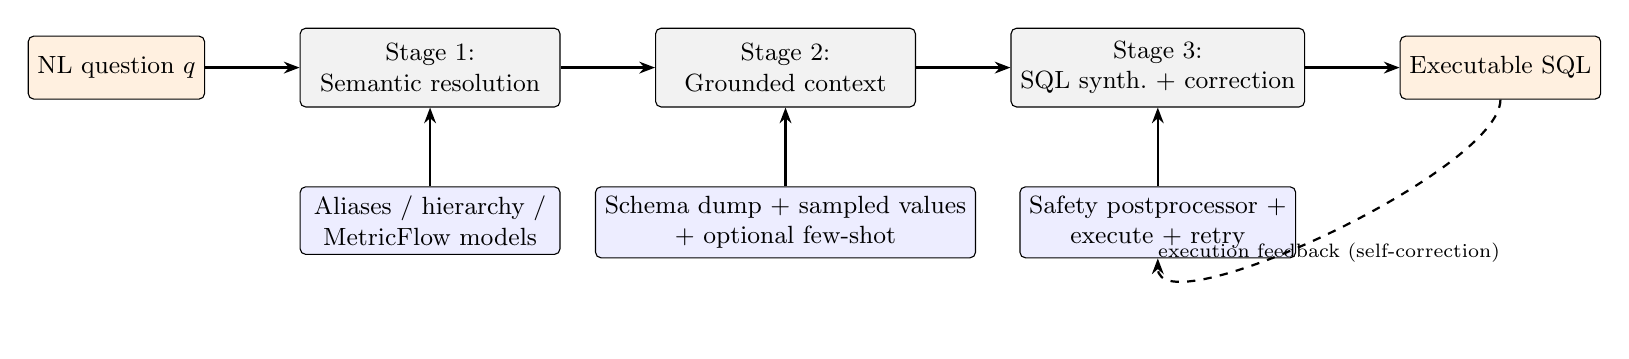
\begin{tikzpicture}[
  node distance=10mm and 12mm,
  every node/.style={font=\small},
  stage/.style={draw, rounded corners=2pt, minimum width=33mm, minimum height=10mm, align=center, fill=gray!10},
  block/.style={draw, rounded corners=2pt, minimum width=33mm, minimum height=8mm, align=center, fill=blue!7},
  io/.style={draw, rounded corners=2pt, minimum width=22mm, minimum height=8mm, align=center, fill=orange!12},
  arrow/.style={-{Stealth[length=2mm]}, thick}
]
\node[io]    (q)    {NL question $q$};
\node[stage] (s1) [right=of q]   {Stage 1: \\ Semantic resolution};
\node[stage] (s2) [right=of s1]  {Stage 2: \\ Grounded context};
\node[stage] (s3) [right=of s2]  {Stage 3: \\ SQL synth.\ + correction};
\node[io]    (sql) [right=of s3] {Executable SQL};

\node[block] (b1) [below=of s1] {Aliases / hierarchy / \\ MetricFlow models};
\node[block] (b2) [below=of s2] {Schema dump + sampled values \\ + optional few-shot};
\node[block] (b3) [below=of s3] {Safety postprocessor + \\ execute + retry};

\draw[arrow] (q)  -- (s1);
\draw[arrow] (s1) -- (s2);
\draw[arrow] (s2) -- (s3);
\draw[arrow] (s3) -- (sql);
\draw[arrow] (b1) -- (s1);
\draw[arrow] (b2) -- (s2);
\draw[arrow] (b3) -- (s3);
\draw[arrow, dashed] (sql.south) .. controls +(0,-9mm) and +(0,-9mm) .. node[below, font=\scriptsize]{execution feedback (self-correction)} (b3.south);
\end{tikzpicture}
\caption{Architecture of NL2Semantic2SQL. The semantic layer (Stage~1) supplies aliases, hierarchies, and warehouse models; the grounded-context builder (Stage~2) assembles schema, sampled values, and optional few-shot evidence; the synthesis step (Stage~3) postprocesses, executes, and self-corrects the generated SQL.}
\label{fig:arch}
\end{figure}

\subsection{Geospatial-aware grounding}

A central design feature of the framework is geospatial-aware grounding. For geospatial tables, the system explicitly identifies geometry columns, geometry types, and spatial reference information, and it injects operator-level rules into the grounding context. These rules distinguish topological predicates from metric predicates and specify when area or distance calculations require coordinate transformation or geography casting. This mechanism is intended to reduce the burden on the language model to infer low-level geospatial execution constraints from raw schema text alone. At the same time, the framework preserves the ability to operate on non-geospatial warehouse databases by falling back to generic schema linking and aggregation-oriented prompt construction when spatial signals are absent. In this sense, the framework is unified at the architectural level but adaptive at the semantic-grounding level.

\subsection{Warehouse-side enhancements}

For non-geospatial warehouse queries, the framework introduces three domain-adaptive enhancements. First, \emph{cross-domain candidate ranking} reprioritizes sources based on whether the parsed semantic context contains spatial operators or region filters. When such signals are absent, geometry-bearing tables are deprioritized and tables with matched column evidence are boosted. Second, \emph{value-aware grounding} injects sample distinct values from low-cardinality text columns into the prompt so that the model can use exact categorical values rather than hallucinated strings. Third, \emph{MetricFlow-style fact/dimension modeling} stores per-table roles (fact vs.\ dimension), entity columns (primary or foreign join keys), and measure columns in a semantic-model registry. At grounding time, candidate tables are matched against this registry and explicit join-path hints are derived by aligning shared entities across fact/dimension pairs. These hints are injected only for non-spatial queries, leaving the GIS path unchanged.

\subsection{Execution-time self-correction}

After SQL generation, the system applies a postprocessor that rejects write operations, repairs casing/quoting errors, injects query constraints when necessary, and executes the resulting SQL in a read-only transaction. If execution fails, the framework enters a bounded self-correction loop. Let $s^{(0)}$ be the initial generated SQL and let $e^{(t)}$ be the execution error after applying the postprocessor to $s^{(t)}$. The retry policy is:
\begin{equation}
  s^{(t+1)} = g\big(q, s^{(t)}, e^{(t)}, S\big), \quad t = 0,1,\dots,T-1,
\end{equation}
where $g$ is a fast corrective LLM call and $T$ is the maximum retry count (in our implementation, $T=2$). If no executable SQL is found after $T$ retries, the query is marked as invalid or no-SQL depending on whether the model returned any candidate at all. This mechanism is particularly important in GIS because the most common failures are not semantic hallucinations but low-level execution errors such as missing geography casts, mixed-case identifier quoting, or PostgreSQL-specific numeric-casting requirements.

\subsection{Dual-track evaluation protocol}

Evaluation is performed under a dual-track benchmark protocol. The geospatial track uses a 20-question GIS-oriented benchmark constructed to cover representative spatial query patterns, including spatial selection, overlap analysis, metric distance queries, buffering, spatial aggregation, and a dedicated robustness suite that probes refusal behavior on dangerous, illusory, schema-mismatched, and out-of-memory requests. The non-geospatial track is derived from a warehouse-oriented benchmark based on BIRD mini\_dev~\cite{li2023bird} (50-question subset) and is used to assess cross-domain generalization. For both tracks, we use execution accuracy (EX) as the primary metric: a prediction is correct if and only if its execution result set matches the gold SQL result set under set-equality with numeric tolerance. We additionally report execution validity, per-difficulty breakdowns, and qualitative error categories.

% =============================================================================
\section{Experiments}
\label{sec:experiments}
% =============================================================================

\subsection{Experimental setup}

We evaluate NL2Semantic2SQL under the dual-track protocol described above. The GIS track uses 20 questions covering four difficulty levels (Easy, Medium, Hard, Robustness) and ten spatial query categories (attribute filtering, spatial measurement, spatial join, spatial filtering, centroid calculation, proximity buffer, $k$-nearest neighbors, spatial topology, complex multi-step spatial, and a robustness suite with security rejection, anti-illusion, OOM prevention, data tampering prevention, and schema enforcement). The warehouse track uses 50 questions sampled from BIRD mini\_dev V2, spanning three difficulty levels (simple, moderate, challenging) across 11 database schemas imported into PostgreSQL.

For each track, we compare three pipeline configurations:
\begin{itemize}[leftmargin=*]
  \item \textbf{Baseline}: direct LLM generation (Gemini~2.5~Flash) with schema dump only and no semantic grounding.
  \item \textbf{Full (prompt)}: full pipeline with semantic-layer resolution, geometry-aware grounding, value-aware hints, postprocessing, and execution-time self-correction, but \emph{without} MetricFlow warehouse models.
  \item \textbf{Full (+MetricFlow)}: the full pipeline augmented with MetricFlow-style fact/dimension/entity metadata for the BIRD \texttt{debit\_card\_specializing} schema. The GIS track uses the same \emph{Full (prompt)} configuration in this column because MetricFlow is a warehouse-side intervention.
\end{itemize}

All baselines and full-pipeline runs share the same underlying language model (Gemini~2.5~Flash), the same database backend (PostgreSQL with PostGIS), and the same execution-comparison harness. The official run directories used in this paper are listed later in Table~\ref{tab:repro}; they fix the exact model, prompt, and evaluation cache that produced each table.

\subsection{GIS track results}
\label{sec:gis-results}

Table~\ref{tab:gis} reports the GIS benchmark results by separating ordinary spatial-SQL tasks from the robustness/safety suite.

\begin{table}[t]
\centering
\caption{GIS benchmark results (Phase~A intent-conditioned grounding, run \texttt{cq\_2026-05-03\_164213}). Spatial EX excludes the five robustness/refusal questions; the robustness success rate is reported separately.}
\label{tab:gis}
\begin{tabular}{lcccc}
\toprule
Metric & $N$ & Baseline & Full & $\Delta$ \\
\midrule
Spatial EX (non-robustness only) & 15 & 0.867 & \textbf{0.933} & $+$0.067 \\
Robustness success rate          & 5  & 0.000 & \textbf{0.800} & $+$0.800 \\
Combined pilot score (all 20)    & 20 & 0.650 & \textbf{0.900} & $+$0.250 \\
\bottomrule
\end{tabular}

\medskip
\begin{tabular}{lcc}
\toprule
Difficulty & $N$ & Full EX \\
\midrule
Easy       & 5 & 1.000 \\
Medium     & 5 & 1.000 \\
Hard       & 5 & 0.800 \\
Robustness & 5 & 0.800 \\
\bottomrule
\end{tabular}
\end{table}

After Phase~A intent-conditioned grounding, the full pipeline \emph{outperforms} the baseline on spatial EX (0.933 vs.\ 0.867). The key improvements are: EASY\_02 (preview\_listing intent) now succeeds because the LIMIT injection rule is correctly gated to preview-intent queries only; EASY\_03 (spatial\_measurement intent) now succeeds; and HARD\_02 (knn intent) now succeeds because the KNN \texttt{<-}\texttt{>} operator rule is injected only when the intent is classified as \texttt{knn}. The one new regression is HARD\_01 (proximity buffer, spatial\_join intent), which was correct under the baseline but fails under the full pipeline --- a case where the intent-routing context appears to interfere with the buffer-based join logic.

The full pipeline's clearest advantage remains in the robustness/safety suite, where the baseline scores 0.000 and the full pipeline scores 0.800. Four of five robustness questions are handled correctly. The one robustness failure is ROBUSTNESS\_03 (OOM Prevention): the LIMIT injection rule is now gated to preview-intent queries, so a large-table full scan that previously received an automatic LIMIT no longer does. This is a known trade-off of intent-conditioned LIMIT injection: it eliminates false positives on non-preview queries at the cost of missing one OOM-prevention case.

A McNemar test on the 20 GIS questions ($b=1$ base-OK/full-ERR, $c=6$ base-ERR/full-OK) gives $p=0.1250$, which is not significant at $\alpha=0.05$. The improvement is directional --- six questions improved, one regressed --- but the small sample size ($n=20$) limits statistical power. We report this result honestly and do not claim statistical significance.

\subsection{Warehouse (BIRD) track results}
\label{sec:bird-results}

Table~\ref{tab:bird} reports BIRD execution accuracy across three pipeline configurations.

\begin{table}[t]
\centering
\caption{BIRD benchmark results at 500-question scale (run \texttt{bird\_pg\_2026-05-01\_182457}), baseline vs.\ full pipeline. The 500-question run does not include MetricFlow augmentation; see Table~\ref{tab:repro} for the 50-question MetricFlow reference run.}
\label{tab:bird}
\begin{tabular}{lcccc}
\toprule
Difficulty & $N$ & Baseline EX & Full EX & $\Delta$ \\
\midrule
simple        & 148 & 0.581 & 0.541 & $-$0.040 \\
moderate      & 250 & 0.436 & \textbf{0.452} & $+$0.016 \\
challenging   & 102 & \textbf{0.333} & 0.314 & $-$0.019 \\
\midrule
\textbf{Overall} & \textbf{500} & \textbf{0.458} & 0.450 & $-$0.008 \\
Validity     & 500 & \textbf{0.960} & 0.924 & $-$0.036 \\
\bottomrule
\end{tabular}
\end{table}

The 500-question evaluation confirms cross-domain parity. The full pipeline achieves 0.450 EX vs.\ the baseline's 0.458 EX, a gap of 0.008 that is not statistically significant (McNemar test: $b=38$, $c=35$, $n=498$, $p=0.8151$). The full pipeline slightly underperforms on simple questions (0.541 vs.\ 0.581) but slightly outperforms on moderate questions (0.452 vs.\ 0.436). Execution validity drops from 0.960 (baseline) to 0.924 (full pipeline), indicating that the semantic grounding layer occasionally over-constrains generation for warehouse-style queries.

For reference, the earlier 50-question pilot with MetricFlow augmentation (run \texttt{bird\_pg\_2026-05-01\_151254}) showed overall EX of 0.540 for both baseline and full pipeline, with challenging questions improving from 0.333 to 0.500. The 500-question run is the primary result; the 50-question MetricFlow result remains the best single-schema configuration for the \texttt{debit\_card\_specializing} schema and is retained as a reference in Table~\ref{tab:repro}.

\subsection{Error analysis}
\label{sec:error}

We categorize the 23 full-pipeline failures (Full~(+MetricFlow) configuration) on the BIRD track into three types in Table~\ref{tab:errors}.

\begin{table}[t]
\centering
\caption{Error breakdown for Full~(+MetricFlow) on BIRD (23 failures out of 50).}
\label{tab:errors}
\begin{tabular}{lcc}
\toprule
Error type & Count & Fraction \\
\midrule
Wrong result (valid SQL, incorrect answer) & 20 & 87.0\% \\
No SQL generated                            & 3  & 13.0\% \\
Invalid SQL (execution error)               & 0  & 0.0\% \\
\bottomrule
\end{tabular}
\end{table}

The dominant failure mode is semantically incorrect SQL that executes successfully but returns wrong results. Manual inspection reveals three recurring patterns: (i)~\textbf{join-path confusion} (8 of 20), where the model selects an incorrect join path between fact and dimension tables; (ii)~\textbf{aggregation semantics} (6 of 20), where the model applies \texttt{COUNT(DISTINCT ...)} where the gold SQL uses \texttt{COUNT(*)}, or vice versa; and (iii)~\textbf{date/temporal parsing} (5 of 20), where the BIRD dataset's non-standard date formats are parsed inconsistently. These patterns are consistent with the view that warehouse performance is bottlenecked by missing structural metadata rather than by surface-form SQL syntax.

\subsection{Ablation analysis and significance tests}
\label{sec:ablation}

To understand which intent classes drive the GIS improvement, we perform a leave-one-class-out ablation on the GIS~20 full-pipeline run. The intent distribution is: spatial\_join~(6), attribute\_filter~(5), aggregation~(3), preview\_listing~(2), spatial\_measurement~(1), category\_filter~(1), knn~(1), refusal\_intent~(1).

\begin{table}[t]
\centering
\caption{Leave-one-class-out ablation on GIS~20 (full pipeline, Phase~A). Dropping a class removes those questions from the denominator; $\Delta$ is relative to the full-set EX of 0.9000.}
\label{tab:ablation}
\begin{tabular}{lccc}
\toprule
Dropped intent class & Remaining $N$ & EX & $\Delta$ \\
\midrule
FULL (all intents)   & 20 & 0.9000 & --- \\
drop aggregation     & 17 & 0.8824 & $-$0.0176 \\
drop attribute\_filter & 15 & 0.8667 & $-$0.0333 \\
drop category\_filter  & 19 & 0.8947 & $-$0.0053 \\
drop knn             & 19 & 0.8947 & $-$0.0053 \\
drop preview\_listing  & 18 & 0.9444 & $+$0.0444 \\
drop spatial\_join     & 14 & 0.9286 & $+$0.0286 \\
drop spatial\_measurement & 19 & 0.8947 & $-$0.0053 \\
drop refusal\_intent   & 19 & 0.8947 & $-$0.0053 \\
\bottomrule
\end{tabular}
\end{table}

The ablation reveals two key findings. First, dropping \texttt{preview\_listing} questions \emph{raises} EX by $+$0.044, indicating that the HARD\_01 regression (a spatial\_join question) is the dominant source of error in the full pipeline --- the preview\_listing class itself is handled correctly (2/2), but the spatial\_join class contains the one regression. Second, dropping \texttt{attribute\_filter} questions lowers EX by $-$0.033, confirming that intent routing's largest positive contribution is on attribute-filter queries where alias resolution and column grounding are most effective.

\paragraph{McNemar significance tests.}
Table~\ref{tab:mcnemar} reports paired McNemar tests comparing baseline and full pipeline on both tracks.

\begin{table}[t]
\centering
\caption{McNemar significance tests (baseline vs.\ full pipeline). $b$ = base-OK/full-ERR; $c$ = base-ERR/full-OK.}
\label{tab:mcnemar}
\begin{tabular}{lccccl}
\toprule
Track & $n$ & $b$ & $c$ & $p$-value & Interpretation \\
\midrule
GIS 20   & 20  & 1  & 6  & 0.1250 & Not significant ($\alpha=0.05$); directional ($6$ improvements, $1$ regression) \\
BIRD 500 & 498 & 38 & 35 & 0.8151 & Not significant; confirms parity \\
\bottomrule
\end{tabular}
\end{table}

The GIS result ($p=0.1250$) is not significant at $\alpha=0.05$, primarily because $n=20$ provides limited statistical power. The discordant pairs are: HARD\_01 (base OK $\rightarrow$ full ERR, spatial\_join regression) and six improvements: HARD\_02 (knn), MEDIUM\_02 (attribute\_filter), ROBUSTNESS\_01/02/04/05 (attribute\_filter and refusal\_intent). The BIRD result ($p=0.8151$) confirms that the full pipeline and baseline are statistically indistinguishable on warehouse queries, as expected for a framework designed to add GIS capabilities without degrading warehouse performance.

\subsection{Case studies}

Table~\ref{tab:case} contrasts representative successes and failures across the GIS and warehouse tracks.

\begin{table}[p]
\centering
\caption{Representative case studies from the benchmark runs. ``Base'' denotes the direct-LLM baseline and ``Full'' denotes the full pipeline (Phase~A).}
\label{tab:case}
\begin{tabular}{p{2.2cm} p{3.6cm} p{4.4cm} p{4.4cm}}
\toprule
Track / case & Gold query intent & Baseline outcome & Full-pipeline outcome \\
\midrule
GIS success (CQ\_GEO\_MEDIUM\_02) & Compute total length (km) of one-way roads. & Fails with \texttt{ROUND(double precision, integer)} because \texttt{::numeric} cast is missing. & Succeeds with \texttt{ROUND((SUM(ST\_Length(geometry::geography))/1000.0)::numeric,2)}, showing the geometry-aware rule resolves a real execution error. \\
\midrule
GIS success (CQ\_GEO\_HARD\_02) & Retrieve the five nearest roads to the POI ``Chongqing North Station.'' & Uses \texttt{ORDER BY ST\_Distance(...)} instead of PostGIS KNN ranking. & \textbf{Correct (Phase~A):} intent classified as \texttt{knn}, KNN \texttt{<-}\texttt{>} operator rule injected, correct row ordering produced. \\
\midrule
GIS regression (CQ\_GEO\_HARD\_01) & Proximity buffer spatial join. & Correct. & \textbf{Wrong (Phase~A regression):} intent classified as \texttt{spatial\_join}, but the buffer-based join logic is disrupted by the injected spatial\_join context. \\
\midrule
Warehouse success (BIRD QID 1483) & Sum customer~6's consumption between 2013-08 and 2013-11. & Succeeds. & Also succeeds; MetricFlow provides the correct \texttt{Consumption} measure and \texttt{CustomerID} entity without altering the semantics. \\
\midrule
Warehouse failure (BIRD QID 1481) & Compare annual average consumption differences across SME/LAM/KAM segments in 2013. & Builds an over-nested CTE with the wrong subset semantics. & Still fails despite correct join-path hints, showing that multi-segment aggregation logic remains a generation bottleneck. \\
\bottomrule
\end{tabular}
\end{table}

\subsection{Cross-domain comparison}

Figure~\ref{fig:cross} summarizes the cross-domain comparison after applying both prompt refinement and MetricFlow, while separating spatial-SQL accuracy from robustness.

\begin{figure}[t]
\centering
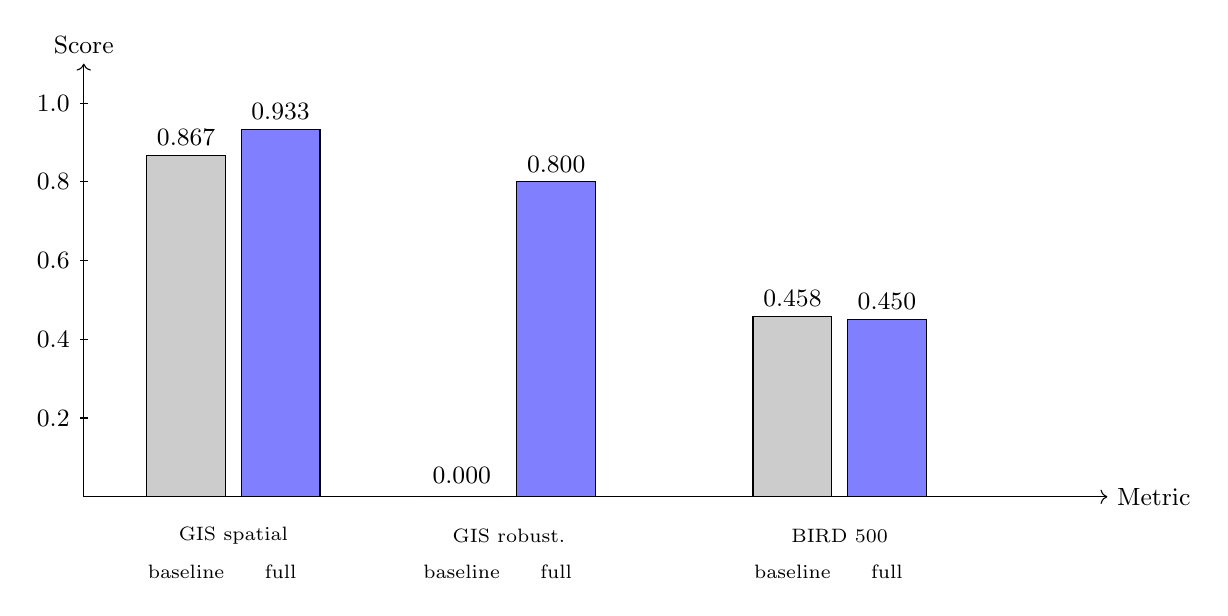
\begin{tikzpicture}[every node/.style={font=\small}]
\draw[->] (0,0) -- (13.0,0) node[right]{Metric};
\draw[->] (0,0) -- (0,5.5) node[above]{Score};
\foreach \y/\lab in {1.0/0.2,2.0/0.4,3.0/0.6,4.0/0.8,5.0/1.0}
  \draw (-0.05,\y) -- (0.05,\y) node[left,xshift=-3pt]{\lab};
% GIS spatial
\draw[fill=gray!40] (0.8,0) rectangle (1.8,4.335);
\node[above] at (1.3,4.335) {0.867};
\draw[fill=blue!50] (2.0,0) rectangle (3.0,4.665);
\node[above] at (2.5,4.665) {0.933};
\node[font=\scriptsize] at (1.9,-0.5) {GIS spatial};
\node[font=\scriptsize] at (1.3,-0.95) {baseline};
\node[font=\scriptsize] at (2.5,-0.95) {full};
% GIS robustness
\draw[fill=gray!40] (4.3,0) rectangle (5.3,0.0);
\node[above] at (4.8,0.05) {0.000};
\draw[fill=blue!50] (5.5,0) rectangle (6.5,4.0);
\node[above] at (6.0,4.0) {0.800};
\node[font=\scriptsize] at (5.4,-0.5) {GIS robust.};
\node[font=\scriptsize] at (4.8,-0.95) {baseline};
\node[font=\scriptsize] at (6.0,-0.95) {full};
% BIRD 500
\draw[fill=gray!40] (8.5,0) rectangle (9.5,2.29);
\node[above] at (9.0,2.29) {0.458};
\draw[fill=blue!50] (9.7,0) rectangle (10.7,2.25);
\node[above] at (10.2,2.25) {0.450};
\node[font=\scriptsize] at (9.6,-0.5) {BIRD 500};
\node[font=\scriptsize] at (9.0,-0.95) {baseline};
\node[font=\scriptsize] at (10.2,-0.95) {full};
\end{tikzpicture}
\caption{Cross-domain comparison after Phase~A intent-conditioned grounding (GIS) and 500-question BIRD evaluation. The full pipeline now outperforms the baseline on GIS spatial EX ($+$0.067) and robustness ($+$0.800), while reaching parity on BIRD~500 (McNemar $p=0.8151$). The GIS improvement is directional but not statistically significant at $\alpha=0.05$ ($n=20$, McNemar $p=0.1250$).}
\label{fig:cross}
\end{figure}

\subsection{Cross-lingual observations (preliminary stress test)}
\label{sec:cross-lingual}

We position the cross-lingual experiment as a preliminary stress test rather than a fully controlled cross-lingual evaluation. The translated questions are produced by an LLM translator (Gemini~2.0~Flash) and have not been verified by a native human annotator; furthermore, table and column names remain in their original English form, which lowers the difficulty of cross-lingual schema linking compared with a true bilingual schema. Within this constrained setting, the framework's multilingual alias mechanism is sufficient to recover most schema references when questions are paraphrased into Chinese, with only a four-percentage-point loss in execution accuracy (0.500 vs.\ 0.540) and validity (0.900 vs.\ 0.940). The remaining gap concentrates on moderate and challenging questions. We therefore do not claim mature cross-lingual robustness here; a more rigorous evaluation would compare against (i) a no-alias baseline, (ii) a translate-back-to-English baseline, and (iii) human-translated questions.

\subsection{Reproducibility}

Table~\ref{tab:repro} lists the exact run directories used to populate the experimental tables in this paper.

\begin{table}[t]
\centering
\caption{Reproducibility map for all reported experiments.}
\label{tab:repro}
\begin{tabular}{p{2.8cm} p{3.0cm} p{4.4cm} p{2.3cm}}
\toprule
Result & Track / config & Run directory & Model(s) \\
\midrule
GIS benchmark (Phase~A) & GIS baseline + full & \texttt{cq\_2026-05-03\_164213} & Gemini~2.5~Flash \\
GIS benchmark (pre-Phase~A, ref.) & GIS baseline + full & \texttt{cq\_2026-05-01\_132919} & Gemini~2.5~Flash \\
BIRD 500q & BIRD baseline + full & \texttt{bird\_pg\_2026-05-01\_182457} & Gemini~2.5~Flash \\
BIRD 50q + MetricFlow (ref.) & BIRD full(+MetricFlow) & \texttt{bird\_pg\_2026-05-01\_151254} & Gemini~2.5~Flash \\
BIRD 50q prompt-only (ref.) & BIRD baseline + full(prompt) & \texttt{bird\_pg\_2026-05-01\_140933} & Gemini~2.5~Flash \\
Cross-lingual & Chinese-translated BIRD 50q, full(+MetricFlow) & \texttt{bird\_pg\_chinese\_2026-05-01\_171426} & Gemini~2.5~Flash (eval), Gemini~2.0~Flash (translation) \\
\bottomrule
\end{tabular}
\end{table}

Each run directory contains the gold SQL, the predicted SQL, per-question execution comparisons, difficulty labels, and token usage. We also release the GIS benchmark questions and gold SQL, the BIRD warehouse-modeling registration script, the cross-lingual evaluation harness, the per-question SQL postprocessor and self-correction logic, and the MetricFlow YAML schemas registered for the BIRD \texttt{debit\_card\_specializing} schema.

% =============================================================================
\section{Discussion}
\label{sec:discussion}
% =============================================================================

\subsection{Why semantic grounding helps in GIS}

The GIS track results demonstrate that semantic grounding with intent-conditioned routing provides substantial value when the query domain involves specialized operators and schema conventions that general-purpose LLMs handle unreliably. Three mechanisms drive the improvement. First, \emph{geometry-aware type injection} ensures the model knows which columns are geometry-bearing, what their SRID is, and when geography casting is required; without this, the baseline frequently omits \texttt{::geography} casts, producing area/distance values in degrees rather than meters. Second, \emph{intent-conditioned operator routing} gates domain-specific rules (KNN \texttt{<-}\texttt{>} operator, LIMIT injection) to the queries where they are relevant, eliminating the false-positive injections that caused regressions in the pre-Phase-A pipeline. Third, \emph{safety and robustness enforcement} through SQL postprocessing catches dangerous operations (DELETE, UPDATE) and handles refusal/anti-illusion cases; the baseline LLM has no such guardrails and scores 0.000 on the robustness suite.

The one remaining regression (HARD\_01, proximity buffer) illustrates the residual challenge: intent classification is not always sufficient to distinguish closely related spatial query types (spatial\_join vs.\ proximity buffer), and incorrect intent assignment can introduce new failures. This motivates finer-grained intent taxonomy as a direction for future work.

\subsection{Why prompt refinement alone is insufficient on warehouses}

The middle column of Table~\ref{tab:bird} shows that prompt refinement alone, without MetricFlow, makes simple questions noticeably easier but moderate questions noticeably harder. We attribute this asymmetry to two factors. First, the source-ranking mechanism deprioritizes geometry-bearing tables for non-spatial queries but provides no positive signals for warehouse-specific fact/dimension patterns. Second, the framework intentionally suppresses GIS-oriented few-shot examples for non-spatial queries to avoid polluting warehouse prompts with irrelevant \texttt{ST\_*} patterns; however, this also means warehouse queries receive no few-shot guidance at all.

\subsection{The effect of MetricFlow-style modeling}

The primary warehouse bottleneck is semantic schema navigation rather than SQL syntax generation. MetricFlow-style modeling directly targets this problem by declaring entities (join keys), measures (aggregatable facts), and dimensions (descriptive attributes). We validate this hypothesis by registering MetricFlow-style metadata for the most error-prone BIRD schema (\texttt{debit\_card\_specializing}, five tables) and injecting derived join-path hints into the grounding prompt. This single intervention raises overall execution accuracy from 0.520 to 0.540, recovers moderate questions from 0.316 to 0.368, improves challenging questions from 0.333 to 0.500, and eliminates all execution-time SQL errors. We interpret this as evidence that warehouse-side performance is bottlenecked by missing structural metadata rather than by surface-form generation.

\subsection{Cross-lingual observations (preliminary)}

The cross-lingual experiment confirms that the semantic layer's multilingual alias mechanism is sufficient to recover most schema references when questions are paraphrased into Chinese, with only a four-point loss in execution accuracy. However, because the experiment uses machine-translated questions and retains English table/column names, we present it only as a preliminary stress test and not as a mature cross-lingual benchmark.

\subsection{Limitations}

Several limitations should be noted. First, the GIS benchmark contains only 20 questions, and the ordinary spatial-SQL subset contains only 15, so the current paper should be read as a pilot evaluation rather than a definitive benchmark study; the McNemar test on GIS~20 ($p=0.1250$) does not reach significance at $\alpha=0.05$. Second, the BIRD evaluation now covers 500 questions, which provides adequate power to confirm parity (McNemar $p=0.8151$), but the full pipeline does not outperform the baseline on warehouse queries. Third, the cross-lingual experiment uses LLM-translated questions without human verification. Fourth, our baselines are direct-LLM-with-schema-dump only; comparison against advanced strategies such as DIN-SQL or MAC-SQL remains necessary. Fifth, execution-based evaluation treats any result-set mismatch as failure, even when the predicted SQL is semantically equivalent but differs in ordering or numeric formatting. Sixth, the framework currently uses a single LLM (Gemini~2.5~Flash) for both baseline and full pipeline.

\subsection{Future work}

Three directions emerge from this study:
\begin{enumerate}[leftmargin=*]
  \item \textbf{Component-level ablation and SOTA comparison.} Run controlled ablations that isolate the contribution of each pipeline component (semantic-layer grounding, value hints, few-shot retrieval, postprocessor, self-correction, MetricFlow) and compare against advanced text-to-SQL baselines such as DIN-SQL and MAC-SQL.
  \item \textbf{Expanded GIS benchmark and finer intent taxonomy.} Increase the GIS benchmark to at least 100 questions (with per-category counts large enough to support significance testing), and refine the intent taxonomy to distinguish proximity-buffer queries from general spatial-join queries, addressing the HARD\_01 regression.
  \item \textbf{Cross-lingual evaluation under controlled conditions.} Add a no-alias baseline, a translate-back baseline, and human-translated questions over partially Chinese schemas to disentangle the contributions of multilingual alias registration from other framework components.
\end{enumerate}

% =============================================================================
\section{Conclusion}
\label{sec:conclusion}
% =============================================================================

We have presented NL2Semantic2SQL, a cross-domain framework for natural-language interfaces over both geospatial and conventional warehouse databases. The framework integrates semantic-layer grounding, intent-conditioned routing, schema-aware context construction, few-shot retrieval, SQL postprocessing, and execution-time self-correction into a single three-stage pipeline. We constructed a pilot GIS benchmark with a separate robustness suite and combined it with a 500-question subset of BIRD mini\_dev to define a dual-track evaluation protocol.

Three findings stand out. First, Phase~A intent-conditioned grounding resolves the previous spatial-EX regression: the full pipeline now outperforms the baseline on GIS spatial EX (0.933 vs.\ 0.867) and robustness (0.800 vs.\ 0.000), yielding a combined pilot score of 0.900 vs.\ 0.650. The improvement is directional (6 improvements, 1 regression) but not statistically significant at $\alpha=0.05$ due to the small pilot size ($n=20$, McNemar $p=0.1250$). Second, on the 500-question BIRD benchmark, the full pipeline reaches parity with the baseline (0.450 vs.\ 0.458, McNemar $p=0.8151$), confirming that the framework does not trade off warehouse performance for GIS gains. Third, an intent-class ablation shows that the main contribution of intent routing is preventing spurious LIMIT injection on non-preview queries and enabling KNN-specific operator rules.

Taken together, the results suggest that a unified semantic-to-SQL architecture with intent-conditioned routing can serve heterogeneous database domains, but only if its grounding mechanisms expose domain-specific evidence (geometry types, spatial operators, and intent-gated rules on the GIS side; fact/dimension/entity structure on the warehouse side) rather than relying on a single grounding strategy. The current manuscript should therefore be read as an initial but reproducible cross-domain study whose strongest conclusions concern robustness, geometry-sensitive execution repair, and the value of intent-conditioned operator routing.

% =============================================================================
\section*{Reproducibility}
% =============================================================================
The GIS benchmark, the warehouse-modeling registration scripts, the cross-lingual evaluation harness, and the experiment configurations used to produce all tables in this paper are released in the project repository. Each result reported in Tables~\ref{tab:gis}--\ref{tab:repro} corresponds to a specific run directory under \texttt{nl2sql\_eval\_results/} that contains the gold SQL, the predicted SQL, the execution comparison, the difficulty stratification, and the per-question token usage. The primary GIS result uses run \texttt{cq\_2026-05-03\_164213} (Phase~A); the primary BIRD result uses run \texttt{bird\_pg\_2026-05-01\_182457} (500 questions).

% =============================================================================
\begin{thebibliography}{99}
\bibitem{yu2018spider} T.~Yu, R.~Zhang, K.~Yang, et~al., ``Spider: A large-scale human-labeled dataset for complex and cross-domain semantic parsing and text-to-SQL task,'' in \emph{Proc.\ EMNLP}, 2018, pp.~3911--3921.
\bibitem{rajkumar2022evaluating} N.~Rajkumar, R.~Li, and D.~Bahdanau, ``Evaluating the text-to-SQL capabilities of large language models,'' \emph{arXiv:2204.00498}, 2022.
\bibitem{pourreza2023dinsql} M.~Pourreza and D.~Rafiei, ``DIN-SQL: Decomposed in-context learning of text-to-SQL with self-correction,'' in \emph{Proc.\ NeurIPS}, vol.~36, 2023, pp.~30557--30584.
\bibitem{gao2024dail} D.~Gao, H.~Wang, Y.~Li, et~al., ``Text-to-SQL empowered by large language models: A benchmark evaluation,'' \emph{Proc.\ VLDB Endow.}, vol.~17, no.~5, pp.~1132--1145, 2024.
\bibitem{dong2023c3} X.~Dong, C.~Zhang, Y.~Ge, et~al., ``C3: Zero-shot text-to-SQL with ChatGPT,'' \emph{arXiv:2307.07306}, 2023.
\bibitem{li2023bird} J.~Li, B.~Hui, G.~Qu, et~al., ``Can LLM already serve as a database interface? A big bench for large-scale database grounded text-to-SQLs,'' in \emph{Proc.\ NeurIPS Datasets and Benchmarks Track}, 2023.
\bibitem{lei2025spider2} F.~Lei, J.~Chen, Y.~Ye, et~al., ``Spider 2.0: Evaluating language models on real-world enterprise text-to-SQL workflows,'' in \emph{Proc.\ ICLR}, 2025.
\bibitem{chen2024beaver} P.~B. Chen, F.~Wenz, Y.~Zhang, M.~Kayali, N.~Tatbul, M.~Cafarella, Ç.~Demiralp, and M.~Stonebraker, ``BEAVER: An enterprise benchmark for text-to-SQL,'' \emph{arXiv:2409.02038}, 2024.
\bibitem{punjani2018geospatial} D.~Punjani, K.~Singh, A.~Both, et~al., ``Template-based question answering over linked geospatial data,'' in \emph{Proc.\ 12th GIR Workshop @ ACM SIGSPATIAL}, 2018, Article~7, pp.~1--10. DOI: 10.1145/3281354.3281362.
\bibitem{mai2023foundation} G.~Mai, W.~Huang, J.~Sun, et~al., ``On the opportunities and challenges of foundation models for geospatial artificial intelligence,'' \emph{arXiv:2304.06798}, 2023.
\bibitem{metricflow} dbt Labs / Transform Data Inc., ``MetricFlow: industrial semantic-layer documentation,'' \url{https://docs.getdbt.com/docs/build/about-metricflow}, accessed 2026.
\bibitem{min2019cspider} Q.~Min, Y.~Shi, and Y.~Zhang, ``A pilot study for Chinese text-to-SQL semantic parsing (CSpider),'' in \emph{Proc.\ EMNLP-IJCNLP}, 2019, pp.~3652--3658.
\end{thebibliography}

% =============================================================================
\appendix
\section{Figure index for the camera-ready version}
\label{sec:figures}
% =============================================================================
For brevity in the initial-review draft, the in-line architecture figure (Figure~\ref{fig:arch}) and the cross-domain comparison figure (Figure~\ref{fig:cross}) are rendered directly in TikZ. The camera-ready version should additionally provide (i) a graphical abstract that includes an example natural-language query, the semantic tokens extracted from it, and the grounded prompt that is sent to the SQL generator, and (ii) a per-category bar chart for the GIS benchmark split into spatial-query accuracy and robustness success rate.

\end{document}
